\documentclass[prl,twocolumn]{revtex4-1}

\usepackage{graphicx}
\usepackage{color}
\usepackage{latexsym,amsmath}
\usepackage{amsfonts}
\usepackage{caption}

\definecolor{linkcolor}{rgb}{1.0,0.647,0.0} %hyperlink
\usepackage[pdftex,colorlinks=true, pdfstartview=FitV, linkcolor= linkcolor, citecolor= linkcolor, urlcolor= linkcolor, hyperindex=true,hyperfigures=true]{hyperref} %hyperlink%

\usepackage{enumitem}
\setlist[itemize]{leftmargin=*}


\setcounter{secnumdepth}{2}

\renewcommand{\thesection}{\arabic{section}}
\renewcommand{\theequation}{\thesection.\arabic{equation}}

\makeatletter
\@addtoreset{equation}{section} % Reset equation counter at each section
\makeatother

\begin{document}

\title{Quantum Optics and Laser, Lab1 - Arecchi's wheel experiment}



\author{Calandra Buonaura Lorenzo}

\date{\today}


\begin{abstract}
In this experiment, we investigate the quantized nature of light by examining its behavior in two distinct quantum states: coherent and thermal light. Our goal is to distinguish coherent laser light's highly correlated photon emission from the random phase and amplitude fluctuations of thermal light using photon statistics.  The study focuses on the discrete photon number distributions characterizing these states, revealing the statistical differences between Poissonian and Bose-Einstein distributions. Furthermore, we take advantage of the intrinsic randomness of quantum events by implementing a Quantum Random Number Generator leveraging coherent light-photon arrival times.
\end{abstract}

\maketitle

\section{Introduction}
The nature of light has been a subject of debate for centuries, dating back to the early scientific discussions between Isaac Newton and Christiaan Huygens; these two great scientist proposed two different views of what light is, completely in contrast with each other. Newton formulated the particle theory of light, proposing that light was composed of small particles, or ``corpuscles", anticipating Einstein conclusion while studying the photoelectric effect. In contrast, Huygens argued that light behaved as a wave, spreading out from a source in all directions; this theory was the most accepted, as phenomena like diffraction and reflection were profoundly understood at the time. This wave-particle duality remained unresolved until the advent of quantum mechanics in the early 20th century, when experiments such as the photoelectric effect and black-body radiation provided compelling evidence for the existence also of a discrete nature of light.

In this experiment, we aim to investigate the granularity of light by examining its particle-like behavior, focusing on two distinct quantum states of light: thermal states and coherent states. Thermal light exhibits random phase and amplitude fluctuations, reflecting a broad distribution of photon energies and is the light produced by natural sources of light or general light bulbs. Coherent light, on the other hand, generated by lasers, has highly correlated photons with constant phase relationships, resulting in a narrow distribution. Through this experiment, we will study the discrete photon distributions of these states, underlying how they can emerge under different physical conditions.

Finally, we'll use the arrival times of our photons to build a Quantum Random Number Generator: this is possible because certain processes, such as the emission or detection of individual photons, are fundamentally random, thanks to quantum mechanics. By measuring the precise time at which each photon arrives, we can extract a truly random sequence of numbers, which relies on the unpredictability of quantum events, making it more secure and less biased compared to classical random number generators, which are often based on deterministic algorithms. The randomness generated from this process has certainly a wide range of applications, from cryptography and secure communications to simulations and complex modeling.

\section{Theoretical framework}
When we are considering a quantum optics experiment, most of the time we have to consider single-photon phenomena and single-photon statistics; this is due to the intrinsic probabilistic nature of quantum mechanics. 

\subsection{Coherent states}
Classically, light can be considered an electromagnetic wave; the most stable type of light that we can imagine is a perfectly coherent light beam, which has a constant angular frequency, phase and amplitude, which is what we would expect from a ideal single-mode laser beam (operating well above threshold)~\cite{pap1}. Thus, having everything constant, there will be no intensity fluctuations and also a time-invariant average photon flux. Now we need to introduce quantum mechanics and the particle nature of light: it could be thought that a beam like this would consist of a stream of photons with regular time intervals between them, but this is not the case, but this is not the case, due to the discrete nature of photons, which implies the presence of statistical fluctuations. Let us consider a light beam of constant power $P$, then the average number of photons within a beam segment of length $L$ is given by:
%
\begin{equation}
    \bar{n} = \frac{\phi L}{c}
\end{equation}
%
where $\phi$ is the photon flux given by:
%
\begin{equation}
    \phi = \frac{P}{h\omega}
\end{equation}

We now subdivide $L$ in $N$ sub-segments of equal length: $N$ is assumed to be large enough that there is only a small probability $p = \frac{\bar{n}}{N}$ of finding a photon in a specific sub-segment and negligible probability of finding two or more~\cite{pap1}. What is the probability $P(n)$ of finding $n$ sub-segments containing exactly $n$ photon within a beam of length $L$ with $N$ sub-segments? It is simply given by the probability of finding $n$ sub-segments with one photon and $N-n$ sub-segments with zero photons, which corresponds to a binomial distribution:
%
\begin{equation}
    P(n) = \frac{N!}{n!(N-n)!} \: p^n \: (1-p)^{N-n}
\end{equation}

Substituting $p = \frac{\bar{n}}{N}$ and taking the limit as $N \rightarrow \infty$, we get that the photon statistics for a coherent light wave with constant intensity are given by:
%
\begin{equation}
    P(n) = \frac{\bar{n}^n}{n!} \: e^{-\bar{n}}, \quad n \in \left[0, \infty\right[
    \label{eq:n_coherent}
\end{equation}
%
which describes a Poissonian distribution~\cite{pap1}, depending on the parameter $\bar{n}$, the average number of photons. The momenta characterizing this distribution can be found in Table~\ref{tab:momenta} in Appendix~\ref{sec:appendix_momenta}.

\subsection{Thermal states}
Most of the natural light sources however cannot be described by coherent light, as they are clearly noisier than a single-mode laser beam, both in the classical (larger variation of intensity) and in the quantum sense (larger photon number fluctuations). The electromagnetic radiation emitted by these sources is usually called thermal light or black-body radiation, which is now a multi-mode radiation; taking into account quantized energy and Planck's law, we can describe the probability of finding $n$ photons in a specific mode by:
%
\begin{equation}
    P_\omega(n) = \frac{1}{1 + \bar{n}} \left( \frac{\bar{n}}{\bar{n} + 1}\right)^n
    \label{eq:n_thermal}
\end{equation}
%
where $\bar{n}$ is given by:
%
\begin{equation}
    \bar{n} = \frac{1}{e^{\frac{\hbar\omega}{k_BT}}-1}
\end{equation}
%
The distribution described by Equation~\eqref{eq:n_thermal} is called Bose-Einstein distribution; it's easy to observe that describes a decreasing exponential with a maximum finite value for $n=0$~\cite{pap1}. The momenta characterizing this distribution can be found in which describes a Poissonian distribution~\cite{pap1}, depending on the parameter $\bar{n}$, the average number of photons. The momenta characterizing this distribution can be found in Table~\ref{tab:momenta} in Appendix~\ref{sec:appendix_momenta}.

\subsection{Quantum Random Number Generator}
\label{sec:qrng_theory}
We can leverage coherent light to build a quantum random generator; the main idea is based on Eisenberg's principle, which states that the product between the uncertainty over time and the uncertainty over energy is always greater than a finite value, meaning that we can't know with infinite precision both energy and time of arrival. We can apply this concept to the photon absorbed by the photodetector: the more precisely the energy of the photon is known (as is the case in a coherent light), the less precisely its arrival time can be predicted. This uncertainty in the time of detection, combined with the probabilistic nature of photon emission, ensures that each photon’s detection is independent of the others and inherently unpredictable.

In particular, for coherent light, photon arrivals follow a Poisson process, where the time intervals between consecutive photon detections are exponentially distributed. The probability density function for the time interval $\Delta T$ between photon arrivals is given by:
%
\begin{equation}
    \label{eq:geometric_distribution}
    f(\Delta T) = \lambda e^{-\lambda \Delta T}
\end{equation}
%
where $\lambda$ represents the average photon detection rate. This exponential distribution arises because, as already pointed out, the emission of photons in a coherent state occurs without any underlying regular pattern or periodicity. In fact, quantum mechanics dictates that each photon has a certain probability of being detected at any given moment, but the precise timing of each event cannot be predicted, which constitutes the perfect ingredient for our quantum random number generator.

But how can we arrive to the QRNG from the arrival time? We need to convert these random times in bit: we can do it considering pairs of consecutive time intervals $\Delta t_i$ and $\Delta t_{i+1}$. For each of these pairs, if $\Delta t_{i+1} > \Delta t_i$, we assign a bit value of 1, otherwise, a 0. If the random number generator is working correctly, we should have about the same occurrences of 0 and 1 in our dataset. After this first step we can group the bits into blocks of 8 to form bytes and convert them to decimal to create our sequence of random numbers: every number in $[0, 255]$ should have the same probability of occurrence, i.e. the resulting byte distribution is expected to be uniform (we could also group every 16, generating number in $[0, 65535]$, but this would require a much larger dataset to be statistically significant). In order to see if the randomness of the sequence is real we need to introduce some tests that take into account the correlation between values in the sequence, which are explained in Appendix~\ref{sec:appendix_random}.


\section{Apparatus}
\begin{figure}
    \centering
    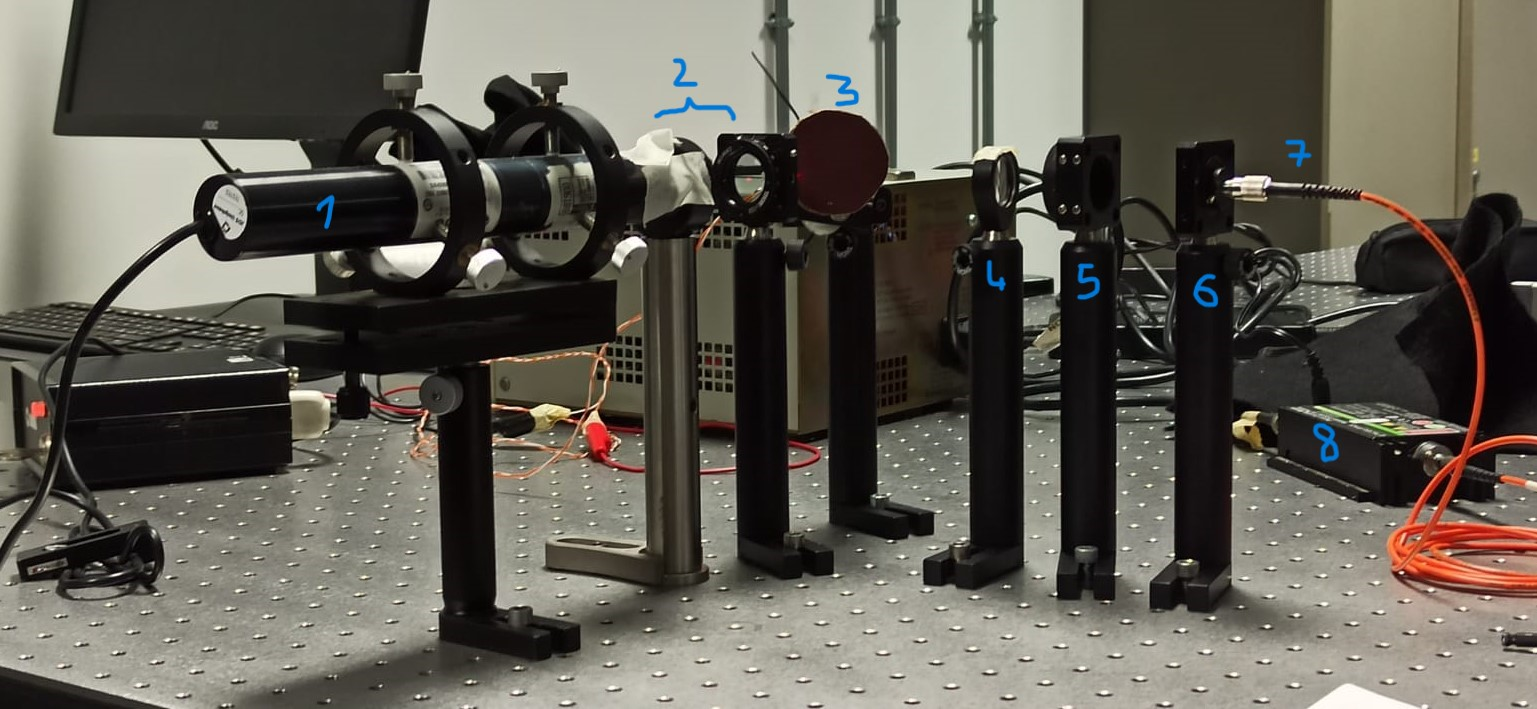
\includegraphics[width=\linewidth]{Images/setup.jpg}
    \caption{Experimental setup, where numbers correspond to the different components explained in the text.}
    \label{fig:setup}
\end{figure}

The setup for this experiment is pretty simple; the main ingredients are a laser, some optical elements (like lenses and polarizers), a sandpaper static or rotating wheel, and a single photon detector. We can see a picture of the whole setup in Figure~\ref{fig:setup}. Obviously, every component has a specific role in the experiment, which is explained in the following:

\begin{enumerate}
    \item \textbf{Gas Tube Laser:} The light source in this experiment is a gas laser, which produces a highly monochromatic (red) and phase-stable beam, ideal for experiments requiring precise control over the light’s properties (coherent light).
    \item \textbf{Polarizers:} A first polarizing filter is placed right in front the exit of the laser beam, to polarize it vertically; a second polarizing filter is placed a bit further in the optical path to control the power of the emitted light. In fact, Malus law states that by adjusting the orientation of the polarizer we can tune the intensity of the light following this relation:
    %
    \begin{equation}
        I = I_0 \cos^2{\theta}
    \end{equation}
    %
    where $\theta$ is the angle between the light's polarization direction (in this case vertical) and the axis of the polarizer. From this relation is clear that we have maximum intensity when the two polarizer have parallel axis and zero intensity when they are perpendicular.
    \item \textbf{Arecchi's Wheel:} The third element of the setup is a sandpaper circle mounted over a rotating device and takes the name of Arecchi's wheel (from Arecchi's experiment, which was one of the first investigating coherent and thermal states). The sandpaper is used for it's roughness, which  introduces fluctuations in the phase and amplitude of the reflected light beam. When the wheel is stationary, the light is simply reflected and remains in a coherent state; on the other hand, when the wheel is in motion, the reflection changes continuously, which disrupt the coherent nature of the laser, introducing random fluctuations that mimic the properties of thermal light.
    \item \textbf{Lens:} The reflected beam then is focused through a convex lens, ensuring that the light is concentrated onto a small area for precise alignment with the next optical system, in particular the optical fiber.
    \item \textbf{Iris:} after the lens, a mechanical iris diaphragm is used to manually control the amount of light entering the optical system, thanks to the adjustable diameter of the iris (we prefer this rather than a polarizer as after the reflection we don't have anymore a polarized beam).
    \item \textbf{Collimator:} The beam then is collected by a collimator, an optical device that collects the divergent light beam from free space and converts it into a parallel beam before coupling it into an optical fiber, ensuring that the light entering the fiber is properly aligned and maintains the necessary intensity for efficient transmission.
    \item \textbf{Optical Fiber:} The optical fiber then transmits the collimated light from the experimental setup to the photon counting system with minimal loss, keeping it isolated from external disturbances.
    \item \textbf{Single Photon Counting Module (SPCM):} Then, the beam enters the single-photon counter, which is the detector on which is based the whole experiment (SPAD, Single-Photon Avalanche Diode). When a photon strikes the detector, it generates a peak of current, which is recorded as a photon detection event, a ``click". From this point on the physical signal becomes digital. An important note to be done is about the working condition this device should be used in: due to its high absorbance, all not necessary light sources must be turned off, to reduce background-noise pollution of the signal and the device should be positioned under a black cloth to reduce even more unwanted clicks.
    \item \textbf{Time Tagger:} The arrival times are recorded thanks to the time tagger, which is an electronic device that logs the exact time at which each photon detection event occurs. The time resolution of the tagger is typically in the nanosecond range, ensuring precise timestamping of each photon event; we must also underline that the time tags of arrival are registered in ``machine units" of  $80.955$ ps.
    \item \textbf{Computer:} Finally, we use the computer to process the data collected by the time tagger and produce the datasets that are used for the analysis of the two quantum state distributions.
\end{enumerate}

All components are securely mounted on an optical table, providing a stable and vibration-isolated environment. This setup minimizes external disturbances, such as mechanical vibrations or air currents, which could introduce significant noise into the photon detection process, falsifying the result of the experiment.
\begin{figure*}[!t]
    \centering
    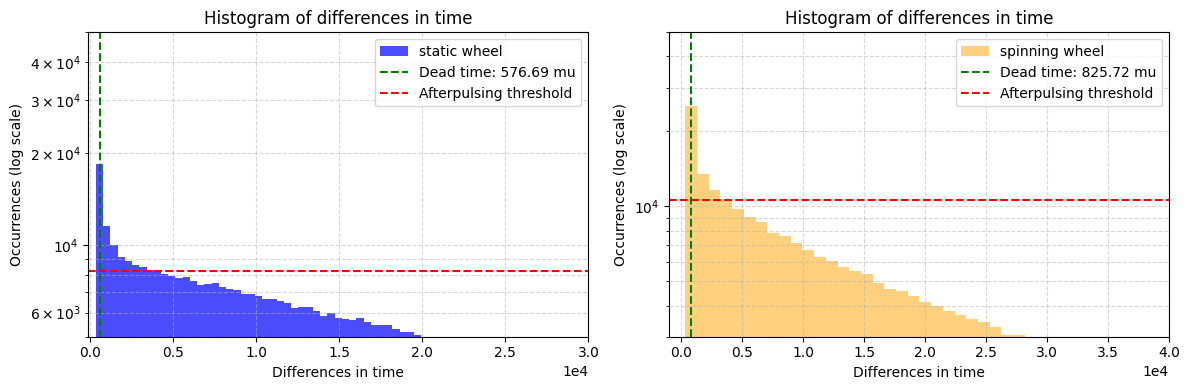
\includegraphics[width=\linewidth]{Images/dead_time.png}
    \caption{Dead time and afterpulsing threshold for static (blue) and spinning (orange) regimes.}
    \label{fig:dead_time}
\end{figure*}

\section{Results}
\subsection{Differences in time}
For both the static and spinning wheel regimes, different dataset have been acquired and compared; the presented result consider one of them. 
The data analysis starts from considering the difference between consecutive time intervals, both for the static and the spinning wheel. This is done as Poissonian processes are characterized by exponentially distributed time intervals
between events (with a constant average rate); thus, we plot it to highlight as in the static case we have a decreasing exponential as expected from Equation~\eqref{eq:geometric_distribution}. Before plotting and proceed with the analysis, we need to consider two main features of the single-photon counter:
\begin{itemize}
    \item \textbf{Dead time:} SPAD detectors experience a dead time of approximately 30 to 50 nanoseconds following each photon detection, during which no further photons can be detected ("no clicks"). As a result, the time histogram generated from photon arrival times will not begin at zero, but rather from a point within this dead-time interval. To perform an accurate fit to the data, it is necessary to account for this delay by shifting the histogram appropriately towards zero, compensating for the dead time and ensuring proper alignment of the detection events.
    
    \item \textbf{Afterpulses:} The SPAD detector used in the experiment has an afterpulsing probability of 0.5\%, meaning that for every detection of a photon, there is a 0.5\% chance that a spurious detection (an afterpulse) will be registered shortly after the initial event (it's a fake click). This occurs due to trapped charge carriers in the detector's material, which can be released after a short delay, mimicking a genuine photon detection. In the context of 1.3 Mclicks, this translates to approximately 7000 afterpulses, which is a non negligible number; to ensure accurate measurements and minimize the influence of these afterpulses, a safety threshold of $3900 \: mu$ is set, beyond which the data can be considered reliable and largely unaffected by afterpulsing artifacts.
\end{itemize}

These two features are depicted for both cases in Figure~\ref{fig:dead_time}, where the histogram representing the differences in times is zoomed in, to highlight them. In the static wheel regime, we get a dead time of $576.69 \: mu = 46.69 \:ns$, in agreement with the expectations; thus, a shifting towards zero will be performed to account for this. Moreover, the lin-log scale highlights even more the afterpulsing in the static regime: we would expect a line with a constant slope, while in the first bins we have an overpopulation, due to the false-clicks of the detector. The $3900 \: mu$ threshold is highlighted in red and it's clear that is a good threshold, as the bins after it follow the expected behaviour. Considering now the spinning wheel instead, the dead time obtained is of $825.72 \: mu = 66.85 \: ns$, still within the same order of magnitude expected; we can observe also in this case the presence of the afterpulsing, even if it's less evident.

The following step, taken into account the previous considerations, is to remove the initial bins to remove afterpulses and shift towards zero to account for dead time. After these simple operations, we can plot again the whole distribution of time interval differences, which is represented in Figure~\ref{fig:diff_time_cleaned}; from the two histograms we can clearly see the exponential behaviour (linear in log scale) of the time differences distribution of the static wheel and the super-exponential (gamma distribution) behaviour in the case of the spinning wheel, as expected. 

\begin{figure*}[!t]
    \centering
    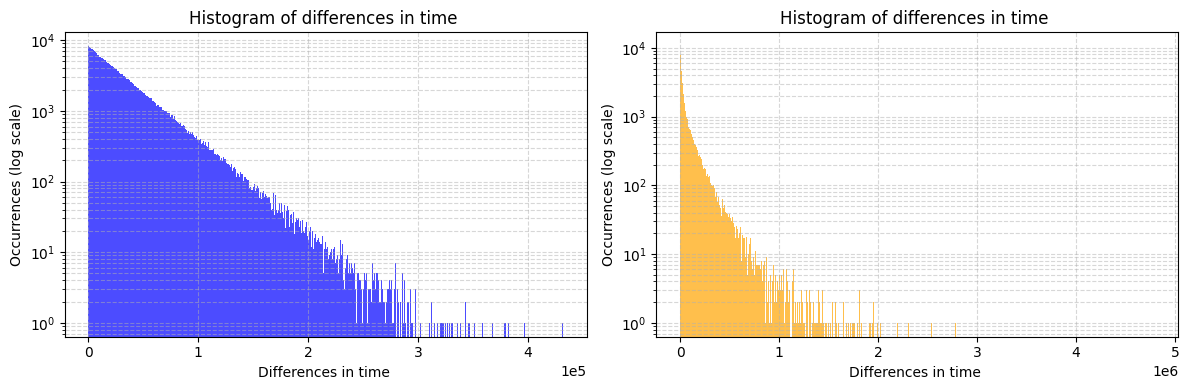
\includegraphics[width=\linewidth]{Images/hist_diff_time_cleaned.png}
    \caption{Time differences distributions: exponential behaviour for the static regime (blue) and super-exponential behaviour for the spinning regime (orange).}
    \label{fig:diff_time_cleaned}
\end{figure*}

\subsection{PDF analysis}
Once the data have been cleaned, we can proceed with the analysis: for each dataset, time tags are grouped in time intervals of suitable duration (in this case we choose $10 \mu s$) and the number of event in each time bin is counted. In this way we are able to produce two histograms and see the actual distribution in the two regimes, as a function of the number of photon detected in each interval. Figure~\ref{fig:distr_fit} depicts the two distributions, completed with a fit; in orange we can see the Bose-Einstein, for thermal light, while in blue the Poissonian, for coherent light. 

\begin{figure}[!b]
    \centering
    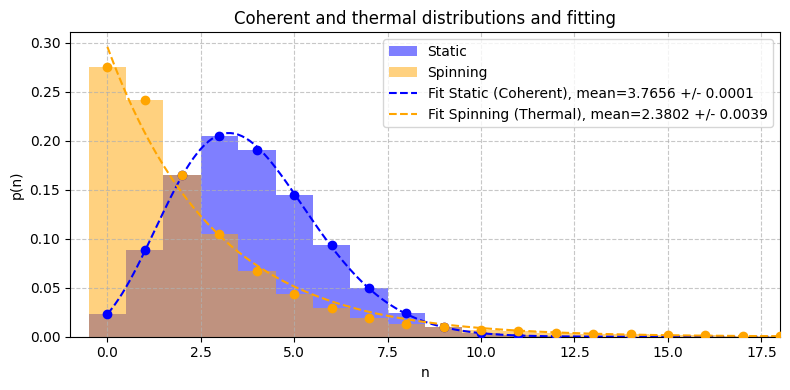
\includegraphics[width=\linewidth]{Images/distr_fit.png}
    \caption{Bose-Einstein and Poissonian distribution, respectively for spinning and static wheel regime.}
    \label{fig:distr_fit}
\end{figure}

Both fits are done using the respective theoretical equations (Equation for the Bose-Einstein and Equation for the Poissonian) and depend on a single parameter, the average photon occupation. For the static wheel regime we get $\bar{n} = 3.7656 \pm 0.0001$, while for the spinning wheel regime we get $\bar{n} = 2.3802 \pm 0.0039$; at first look this values seem plausible, as $\bar{n}$ is smaller for thermal light (due to the fact that the Bose-Einstein distribution has its maximum in $n = 0$). In order to see whether the fits and the data are actually comparable is necessary to have a look to some statistics of the distributions, comparing the numerical result to the expected (analytical) result; Appendix~\ref{sec:appendix_momenta} summarizes why we use these statistics and how they are related to distribution momenta. 

\begin{table}[htbp]
    \centering
    \begin{tabular}{|c||c||c|}
        \hline
        \textbf{Statistic} & \textbf{Static Wheel} & \textbf{Spinning Wheel} \\
        \hline
        \hline
        Mean               & $3.779 \pm 0.0051$                 & $2.2739 \pm 0.0087$                     \\ 
        \hline
        Variance           & $3.8481 \pm 0.0154$                & $8.0133 \pm 0.0818$                     \\ 
        \hline
        Skewness           & $0.5329 \pm 0.0525$                & $2.5404 \pm 0.0905$                     \\ 
        \hline
        Kurtosis           & $3.2821 \pm 0.3773$                & $12.4165 \pm 1.0364$                    \\ 
        \hline
    \end{tabular}
    \caption{Numerical statistics for static and spinning wheel regimes (with errors).}
    \label{tab:numerical}
\end{table}

\begin{table}[htbp]
    \centering
    \begin{tabular}{|c||c||c|}
        \hline
        \textbf{Statistic} & \textbf{Static Wheel}  & \textbf{Spinning Wheel}  \\ 
        \hline
        \hline
        Mean               & $3.7656 \pm 0.0001$                & $2.3755 \pm 0.0085$                     \\ 
        \hline
        Variance           & $3.7656 \pm 0.0001$                & $8.0183 \pm 0.0004$                                \\ 
        \hline
        Skewness           & $0.5153 \pm 0.0001$                & $2.0309 \pm 0.0045$                                \\ 
        \hline
        Kurtosis           & $3.2656 \pm 0.0001$                & $9.1247 \pm 0.0080$                                \\ 
        \hline
    \end{tabular}
    \caption{Analytical statistics for static and spinning wheel regimes (with errors).}
    \label{tab:analytical}
\end{table}

Table~\ref{tab:numerical} and Table~\ref{tab:analytical} report the values of the statistics (mean, variance, skewness and kurtosis) for the two regimes, computed in the numerical and in the analytical way, respectively. The errors have been computed in two different ways: for the analytical part, a simple error propagation has been used. For the numerical part, instead, bootstrapping has been applied, which is a statistical technique used to estimate the distribution of a statistic by repeatedly sampling with replacement from the original dataset. This involves generating multiple resampled datasets of the same size, calculating the desired statistic for each, and then constructing an empirical distribution from these statistics. As we can see, a general agreement is present, even if for the spinning wheel the error propagation is important and thus skewness and kurtosis diverge from the expected values. 

\subsection{Quantum random number generator}
\begin{figure}
    \centering
    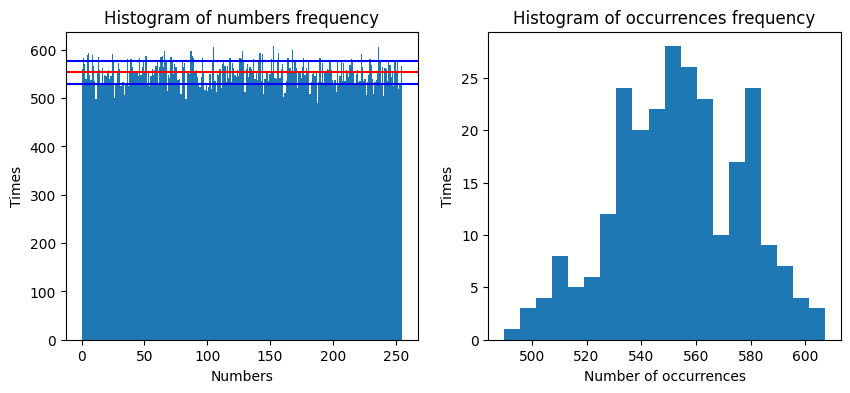
\includegraphics[width=\linewidth]{Images/qrng_stats.png}
    \caption{Quantum random number sequence analysis}
    \label{fig:qrng_stats}
\end{figure}

\begin{figure}[!b]
    \centering
    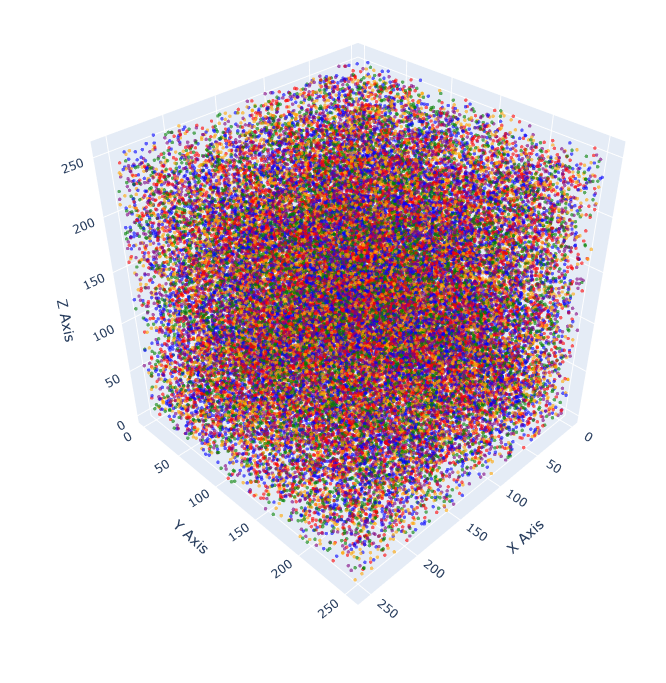
\includegraphics[width=0.8\linewidth]{Images/QRNG.png}
    \caption{Cloud of points, generated using the QRN sequence from the experiment.}
    \label{fig:QRNG}
\end{figure}

The quantum random number generator is based on a quantum random number list, which can be obtained following the basic ideas explained in Section~\ref{sec:qrng_theory}. After building the bits list, grouping it into bytes and then transforming to decimal, we can analyze it in order to see whether it is really completly random or not. Figure~\ref{fig:qrng_stats} illustrates two histograms. The first histogram displays the frequency of each decimal number in the dataset, while the second histogram represents the occurrences of these frequencies, showing how many times each frequency value appears in the first histogram. From these histograms, we can see that the number distribution is pretty much uniform (the mean is $127.33$) and the occurrences distribution is peaked in the middle, with low-population tails. 

This is the first step in order to see if the QRNG is working correctly; we can visualize it also in 3D (considering the numbers in triplets, simulating 3D coordinates), as in Figure~\ref{fig:QRNG}. The cloud is dense and doesn't present any visible pattern, which is another point in favour of our thesis (also rotating it nothing strange appears). 

But how can we be sure that this sequence is truly random? Infact, we obtained a good approximation of a uniform ditribution, but we don't know anything about the intrinsic correlation of values. This is clear when we compare the same histograms computed for a Pseudo-Random Number Generator (using \texttt{numpy.random} module), which we already know has some correlations inside its sequence. Figure~\ref{fig:prng_stats} presents the same two histograms as before and we can notice how the same conclusion can be done: the first is similar to a uniform distribution (the mean is $127.26$) and the second is peaked around the mean number of occurrences, as expected. Thus, we need to investigate more in order to understand if our quantum random number list is truly random or has some intrinsic correlation. In order to do so, we leverage some statistical methods developed to study the randomness of a
number sequence, based on the ENT module (see Appendix~\ref{sec:appendix_random}). When we apply these method to our quantum random number sequence, the output we get is:
\begin{figure}[!t]
    \centering
    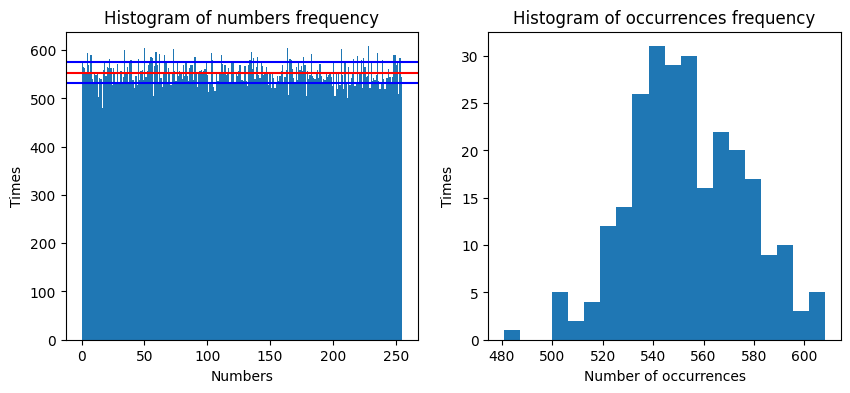
\includegraphics[width=\linewidth]{Images/prng_stats.png}
    \caption{Pseudo-random number sequence analysis}
    \label{fig:prng_stats}
\end{figure}

\begin{enumerate}
    \item \texttt{Entropy: 0.999998 bits per bit.}
    \item \texttt{Optimum compression would reduce the size of this 1133472 bit file by 0 percent.}
    \item \texttt{Chi-square distribution for 1133472 samples: 3.91, randomly exceeding this value 4.79 percent of the time.}
    \item \texttt{Arithmetic mean value of data bits: 0.4991 (0.5 = random).}
    \item \texttt{Monte Carlo value for Pi: 3.132548488 (error 0.29 percent).}
    \item \texttt{Serial correlation coefficient: 0.001281 (totally uncorrelated = 0.0).}
\end{enumerate}

On the other hand, when applied to a pseudo-random number sequence, the output we get is:
\begin{enumerate}
    \item \texttt{Entropy: 0.337119 bits per bit.}
    \item \texttt{Optimum compression would reduce the size of this 9067776 bit file by 66 percent.}
    \item \texttt{Chi-square distribution for 9067776 samples: 6943909.07, randomly exceeding this value less than 0.01 percent of the time.}
    \item \texttt{Arithmetic mean value of data bits: 0.0625 (0.5 = random).}
    \item \texttt{Monte Carlo value for Pi: 4.000000000 (error 27.32 percent).}
    \item \texttt{Serial correlation coefficient: 0.400053 (totally uncorrelated = 0.0).}
\end{enumerate}

As we can clearly see, all the results for the quantum random number sequence suggest a high value of randomness, with near-zero correlation, while those obtained for the pseudo-random number sequence reveal the existence of an intrinsic correlation, which makes the sequence not truly random.

\section{Conclusions}
In this study, we investigated the statistical properties of two different quantum states, coherent and thermal light; we leveraged the Arecchi's wheel setup to generate both states without changes in the laser or the optical elements, simply using a static or a spinning wheel. The analysis of the collected dataset revealed significant differences in the respective distributions, in agreement with the expectation; the time differences analysis demonstrated indeed the exponential decay in the static regime and a super-exponential behavior in the spinning regime.

Furthermore, the comparative analysis of the two regimes, through numerical and analytical statistics, showcased a general agreement, affirming the validity of the results obtained. We also noticed that for the spinning regime the error propagation in the formula is not negligible, which causes the skewness and the kurtosis in this case to diverge from the expected value; surely, an larger dataset would permit a better evaluation of the mean and, consequently, of the other momenta.

The evaluation of the quantum random number generator (built over the coherent photon arrival times) revealed a high degree of randomness, supported by robust statistical tests indicating near-zero correlation. In contrast, the pseudo-random number generator exhibited significant correlation, confirming that it does not produce truly random sequences. Thus, a setup like the one present in this experiment could be a starting point to develop new technologies to produce truly random sequences.


\section{Appendix}
\subsection{Distributions' Momenta}
\label{sec:appendix_momenta}
In statistics, the momenta of a distribution provide critical insights into its shape and characteristics. For discrete random variables, the \(n\)-th moment about the origin is defined as the expected value of the \(n\)-th power of the variable, which mathematically reads as:
%
\begin{equation}
    \mu_n = \mathbb{E}[X^n] = \sum_{k=0}^{\infty} k^n P(X = k),
\end{equation}

where \(P(X = k)\) is the probability mass function of the random variable \(X\). Most of the times, we are interested in quantities strictly related to the momenta rather the momenta themselves, which are more informative about the distribution. After the mean (first momentum), we usually care about variance, skewness and kurtosis:

\begin{itemize}
    \item \textbf{Variance:} 
    Measures the dispersion of a set of values relative to their mean. It is the second central moment and is defined as:
    \begin{equation}
        \text{Variance} = \sigma^2 = \mathbb{E}[(X - \mu)^2] = \mu_2',
    \end{equation}
    where \(X\) is the random variable, \(\mu\) is the mean, and \(\mu_2'\) is the second moment about the origin. A higher variance indicates greater spread in the data, while a smaller variance indicates a more peaked distribution.

    \item \textbf{Skewness:} 
    Quantifies the asymmetry of a probability distribution. It is the third standardized moment, defined as:
    \begin{equation}
        \text{Skewness} = \gamma_1 = \frac{\mathbb{E}[(X - \mu)^3]}{\sigma^3} = \frac{\mu_3'}{\sigma^3},
    \end{equation}
    where \(\mu_3'\) is the third moment about the origin. A skewness of zero indicates a symmetric distribution, while positive or negative values indicate right or left skewness, respectively.

    \item \textbf{Kurtosis:} 
    Measures the "tailedness" of a distribution, indicating the presence of outliers. It is defined as the fourth standardized moment:
    \begin{equation}
        \text{Kurtosis} = \gamma_2 = \frac{\mathbb{E}[(X - \mu)^4]}{\sigma^4} = \frac{\mu_4'}{\sigma^4},
    \end{equation}
    where \(\mu_4'\) is the fourth moment about the origin. A normal distribution has a kurtosis of 3, so most of the time we consider the excess kurtosis (subtracting 3) to assess whether a distribution is more or less peaked than normal.

\end{itemize}

Table~\ref{tab:momenta} summarizes the value of these quantities for the Poissonian and the Bose-Einstein distributions, which are used to compare the expected values (based on the results from the fit) and the numerical values obtained from the data.

\begin{table}[h!]
    \centering
    \begin{tabular}{|c||c||c|}
        \hline
        \textbf{Statistic} & \textbf{Poissonian} & \textbf{Bose-Einstein} \\
        \hline
        \hline
        Mean & $\mu$ & $\mu$ \\
        \hline
        Variance $(\sigma)$ & $\mu$ & $\mu + \mu^2$ \\
        \hline
        Skewness & $1/\sqrt{\mu}$ & $(1 + 2\mu)/\sqrt{\sigma}$ \\
        \hline
        Kurtosis & $1/\mu$ & $(6\mu + 6\mu^2 + 1)/\sigma$ \\
        \hline
    \end{tabular}
    \caption{Analytical form of momenta for Poissonian and Bose-Einstein distributions.}
\label{tab:momenta}
\end{table}

\subsection{Statistical methods for randomness analysis}
\label{sec:appendix_random}
The statistical methods to study the randomness of a number sequence are based on the ENT module, which is a ``Pseudorandom Number Sequence Test Program"~\cite{fourmilab}. Here we'll explain the main principle of each method, highlighting good and bad results. 

\begin{itemize}
    \item \textbf{Entropy}: Measure of the information density in a sequence of data (often expressed in bits per character or bits per symbol), it quantifies the unpredictability or randomness of a sequence, with higher entropy corresponding to a higher degree of randomness. The formula for entropy $H$ is:
    %
    \begin{equation}
        H = -\sum_{i=1}^{n} p_i \log_2 p_i
    \end{equation}
    %
    where $p_i$ is the probability of occurrence of the $i$-th symbol in the sequence. Entropy close to the theoretical maximum indicates that the data is highly random, while lower entropy suggests a more structured or predictable sequence.

    \item \textbf{Chi-Square Test}: Statistical method used to assess whether the distribution of elements in a data sequence deviates from what would be expected in a random sequence. It compares the observed frequencies of data points to the expected frequencies under the assumption of uniform randomness. The chi-square statistic is given by:
    %
    \begin{equation}
        \chi^2 = \sum_{i=1}^{k} \frac{(O_i - E_i)^2}{E_i}
    \end{equation}
    %
    where $O_i$ is the observed frequency of the $i$-th event and $E_i$ is the expected frequency. The result of the test can be expressed as a percentage, indicating the probability that the observed distribution could arise from a truly random process: values far from 50\% suggest non-randomness.

    \item \textbf{Arithmetic Mean}: Basic statistical measure that computes the average value of all the bytes (or bits) in a sequence; for a truly random sequence, the mean should be approximately 127.5 when considering bytes (ranging from 0 to 255) or 0.5 when considering bits (0 or 1). Deviations from the expected mean can indicate systematic biases or non-randomness.

    \item \textbf{Monte Carlo Method for Pi}: This method utilizes randomly generated data to estimate the value of $\pi$. Each successive sequence of six bytes (or other length of interest) is treated as coordinates $(x, y)$ within a square, and the fraction of points falling inside the inscribed circle is used to approximate $\pi$. The value of $\pi$ is approximated as:
    %
    \begin{equation}
        \pi \approx 4 \times \frac{\text{number of points inside the circle}}{\text{total number of points}}
    \end{equation}
    %
    For sufficiently large data sets, the approximation converges to the true value of $\pi$ only if the data is random.

    \item \textbf{Serial Correlation Coefficient}: Measures the extent to which each value in a sequence is related to its predecessor and is calculated as:
    %
    \begin{equation}
        \rho = \frac{\sum_{i=1}^{N-1} (x_i - \mu)(x_{i+1} - \mu)}{\sum_{i=1}^{N} (x_i - \mu)^2}
    \end{equation}
    %
    where $x_i$ are the data points, $\mu$ is the mean of the sequence, and $N$ is the total number of points.  For a random sequence, this correlation should be close to zero, indicating no dependence between consecutive elements; on the other hand, a coefficient close to 1 or -1 indicates strong correlation (or anti-correlation), which suggests the sequence is not random.
\end{itemize}

\section{Code}
All the data and the code for the data analysis can be found in this public Github repository: \href{https://github.com/Kallo27/QOL}{https://github.com/Kallo27/QOL}

\begin{thebibliography}{99}

\bibitem{pap1}
  M. Fox, \textit{Quantum Optics - An Introduction}, Oxford University Press (2006).

\bibitem{fourmilab}
  J. Walker, \textit{HotBits: Genuine Random Numbers from Radioactive Decay}, \href{https://www.fourmilab.ch/random/}{https://www.fourmilab.ch/random/}.

\end{thebibliography}

\end{document}